\documentclass[UTF8]{report}
\usepackage{graphicx}
\usepackage{xetexko}

\title{%
    <컴퓨터프로그래밍 3> 실습 보고서 \\ 
    \large [제 03 주] 마방진}
\author{201704150 허강준}
\date{\today}


\begin{document}
    \maketitle
    \tableofcontents

    \chapter{프로그램 설명서}
        본 보고서에서는 객체를 사용하지 않고 마방진을 처리하는 프로그램에 대해 기술한다.

        \section{프로그램의 전체 설계 구조 (MVC 등)}
            
            \paragraph{%
                \normalfont 1, 2주차에서 사용했던 기존의 프레임워크를 재활용하며, 마방진 계산의 처리를 위해 \texttt{MagicSquare} 모듈을 도입하였다. 최대 처리 가능 크기(\texttt{MAX\_ORDER})를 도입하도록 한 것에 따라, Visual Studio에서 설정한 기본 스택 사이즈인 16KB를 넘을 수 있으므로 전역 변수 영역에 마방진 배열을 선언하였다.
            }

            \paragraph{%
                \normalfont 마방진을 위한 객체를 사용하지 않으므로, 마방진을 표현하기 위해 99x99 크기의 배열을 전역으로 선언하였다. \texttt{App\_Start} 에 지역번수로서 선언하지 않은 이유는 위에서 언급한 스택 사이즈의 문제이며 이는 프로젝트 설정 등을 통하여 해결할 수 있으나 채점 과정에서 문제가 될 수 있으므로 정석을 따르도록 한다.
            }
            
        \section{함수 설명서}

            \paragraph{MACRO:\texttt{BOARD\_ARG(x)}}
            \paragraph{%
                \normalfont 2차원 배열을 인자로 넘기기 위하여 \texttt{int x[MS\_MAX\_ORDER]} 의 꼴을 반복하는 것은 코드 가독성을 해칠 수 있으므로, 매크로로 처리하도록 하였다.
            }
            
            \paragraph{\texttt{MagicSquare\_orderIsValid(int order)}}
            \paragraph{%
                \normalfont 마방진의 차수는 3 이상의 홀수에 대해서, 그리고 99로 정의된 최대 차수보다 작아야 한다. 따라서 이 조건을 만족하지 못할 경우 \texttt{false}를 리턴한다.
            }

            \paragraph{\texttt{MagicSquare\_solve(BOARD\_ARG(board), unsigned int order)}}
            \paragraph{%
                \normalfont 실습 자료에서 제시한 알고리즘에 따라 마방진을 풀이한다. 객체를 사용하지 않으므로 풀이할 차수를 인자로 제공한다.
            }

            \paragraph{\texttt{MagicSquare\_clear(BOARD\_ARG(board), unsigned int order)}}
            \paragraph{%
                \normalfont 마방진 풀이 프로그램은 프로그램이 종료될 때 까지 반복할 수 있으므로, 기존에 남아있는 마방진 데이터를 삭제한다.
            }

        \section{종합 설명서}

            \paragraph{%
                \normalfont 마방진은 모든 행과 열, 그리고 대각선의 합이 전부 동일하도록 수를 정사각행렬에 배치한 것이다. 1부터 $n^2$ 까지의 자연수가 차례로 배치된다
            }

            \paragraph{%
                \normalfont 본 프로그램에서는 실습 자료에서 제시된 알고리즘을 사용하였으며 그 방법은 다음과 같다:
            }

            \begin{itemize}
                \item 첫번째 행의 중앙 열 s부터 시작한다. (차수 n에 대해 $s = n >> 1$, >>는 우측 쉬프트 연산)
                \item 오른쪽 위로 올라가며 1씩 증가한다.
                \item 만일 채우고자 하는 칸에 이미 값이 채워진 경우 현재 칸의 바로 아래 칸을 채운다.
                \item 이때 행렬을 벗어날 경우, 다음 규칙에 따라 다음 칸을 선정한다:\\
                      \begin{itemize}
                          \item 위쪽 방향일 경우 마지막 행으로 이동한다.
                          \item 아랫쪽 방향일 경우 처음 행으로 이동한다.
                          \item 오른쪽 방향일 경우 첫 열로 이동한다.
                          \item 왼쪽 방향일 경우 마지막 열로 이동한다.
                      \end{itemize}
            \end{itemize}
                
    \chapter{프로그램 장단점/특이점 분석}
        \section{객체를 사용하지 않고 짠 경우에 대해}
            \paragraph{%
                \normalfont 본 프로그램에서는 객체를 사용하지 않고 마방진을 구현하였다. 그러나 이 경우 마방진 관련 함수를 호출할 때마다 차수를 인자로 넘겨주어야 하는 문제가 발생한다. 물론 인자 외에도 차수 정보를 획득하는 방법은 여러가지가 있으나, 추가적인 Boilerplate 등을 사용하지 않으면서 최대한 가독성을 보장하는 방법으로는 인자로 넘기는 것이 최적이라고 판단된다.
            }

        \section{매크로 \texttt{BOARD\_ARG}}
            \paragraph{%
                \normalfont 배열은 포인터와 동치되어 포인터를 통해 인자로 넘겨 사용할 수 있으나, 배열과 포인터는 근본적으로 다르므로 배열임을 명시하여 인자로 넘기는 것이 바람직하다. 그러나 다차원 배열을 인자로 넘겨 사용할 경우 코드의 가독성을 저해할 수 있으므로 매크로를 사용함이 바람직하다. 이는 추후 객체를 사용한 마방진에서 객체의 포인터를 넘기는 식으로 사용할 수 있을 것이다.
            }

        \section{차수 판단의 문제}
            \paragraph{%
                \normalfont \texttt{MagicSquare\_orderIsValid} 는 차수가 가능한 모든 조건대 대해서 참/거짓 판단만 하므로 개별 위배 조건에 대한 판단은 할 수 없다. 따라서 App 메인 플로우에서 유효한지 여부에 대한 검사 이후 개별 위배 조건에 대해 AppView를 호출하는 식으로 작성하였다.
            }
        
        \chapter{실행 결과 분석}
            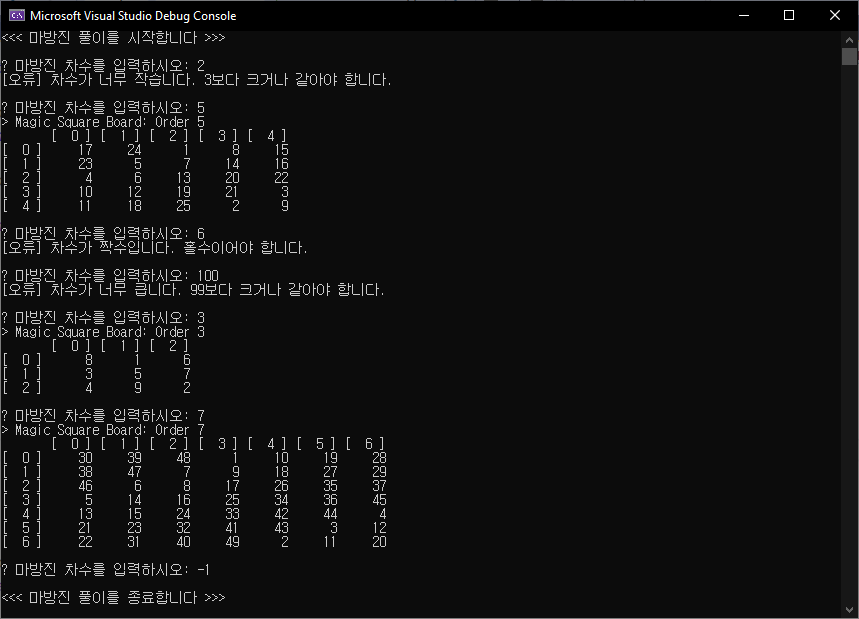
\includegraphics[width=\textwidth]{test_result.png}
            \section{입력과 출력}
                실습 자료에서 제시된 입력을 사용하였으며 모든 경우에 대해 정상적으로 처리됨을 확인하였음.
            \section{결과 분석}
                실습 자료에서 제시된 출력과 동일함을 확인하였음.
    
        \chapter{소스코드}
            소스코드는 제출된 압축파일에 같이 동봉되어있으며 GitHub (0x00000FF/CNUCSE-Computer-Programming-III-2020-Spring) 에서도 열람할 수 있다.
\end{document}